\documentclass{article}

\usepackage{jmlr2e}
\usepackage{natbib}
\usepackage{hyperref}
\usepackage{amssymb,amsmath,epsfig}
\usepackage{caption}
\usepackage[utf8]{inputenc}
\usepackage[french]{babel}
\usepackage{lipsum}
\sloppy
\hypersetup{
    colorlinks=true,
    linkcolor=blue,
    filecolor=magenta,      
    urlcolor=cyan,
    pdftitle={Overleaf Example},
    pdfpagemode=FullScreen,
}
%%%%%%%%%%%%%%%%%%%%%%%

\editor{Machine Learning Avancé (2023-2024)}

\begin{document}

\title{Neural Machine Translation by Jointly Learning to Align
and Translate}

%% Group authors per affiliation:

\author{\name JAMIL Alhussein \email alhussein.jamil@polytechnique.edu \\
       \addr Master Ingénierie des Systèmes Intelligents \\
       Sorbonne Université\\
       Paris, France}
\maketitle

% Abstract section

\begin{abstract}

% \textbf{As part of our Advanced Machine Learning project, we embarked on the re-implementation of a neural machine translation system outlined in a research paper. This model serves the purpose of translating sentences from a source language to a target language. Its architecture is composed of three key elements: an encoder, responsible for processing and encoding input sentences into variable-length vectors; a decoder, tasked with generating translated sentences in the target language; and an attention mechanism positioned between the encoder and decoder. This attention mechanism plays a crucial role in considering the contextual information of each word in the input sentence, taking into account both preceding and succeeding words for a more comprehensive translation.}
\textbf{Neural machine translation (NMT) is a recent approach to machine translation that has shown promising results in terms of translation quality. In this report, we present our implementation of a neural machine translation model that jointly learns to align and translate, based on the work of Bahdanau et al. (2015). We evaluate our model on the English-French translation task using the WMT14 dataset, and compare its performance to a baseline model that uses a basic encoder-decoder architecture. Our results show that the proposed approach outperforms the baseline model in terms of BLEU score and alignment quality.}
\end{abstract}




% INTRO section
\section{Introduction}
\label{sec:intro}

\textbf{}
Machine translation is the task of automatically translating text from one language to another. Traditional approaches to machine translation rely on statistical models that learn to map source language sentences to target language sentences based on large parallel corpora. However, these models often suffer from the problem of data sparsity, and require extensive feature engineering to achieve good performance. In recent years, neural machine translation (NMT) has emerged as a promising alternative to traditional statistical machine translation. NMT models use neural networks to learn to translate directly from source to target language, without relying on hand-crafted features or alignment models. In this report, we present our implementation of a neural machine translation model that jointly learns to align and translate, based on the work of Bahdanau et al. (2015). We aim to assess the performance of our model on the English-French translation task with the WMT14 dataset, and contrast its results with those of a baseline model employing a simple encoder-decoder architecture. Our objective is to not only gauge the effectiveness of the proposed approach but also to delve into the model's behavior through a detailed analysis of its alignment patterns. The full implementation is available on github \href{https://github.com/alhussein-jamil/MLA_Project}{Neural Machine Translation by Jointly Learning to Align and Translate paper implementation} 
\newpage
% METHODE section
\section{Method}
\label{sec:methode}
\subsection{Architecture}

\begin{figure}[h]
    \centering
    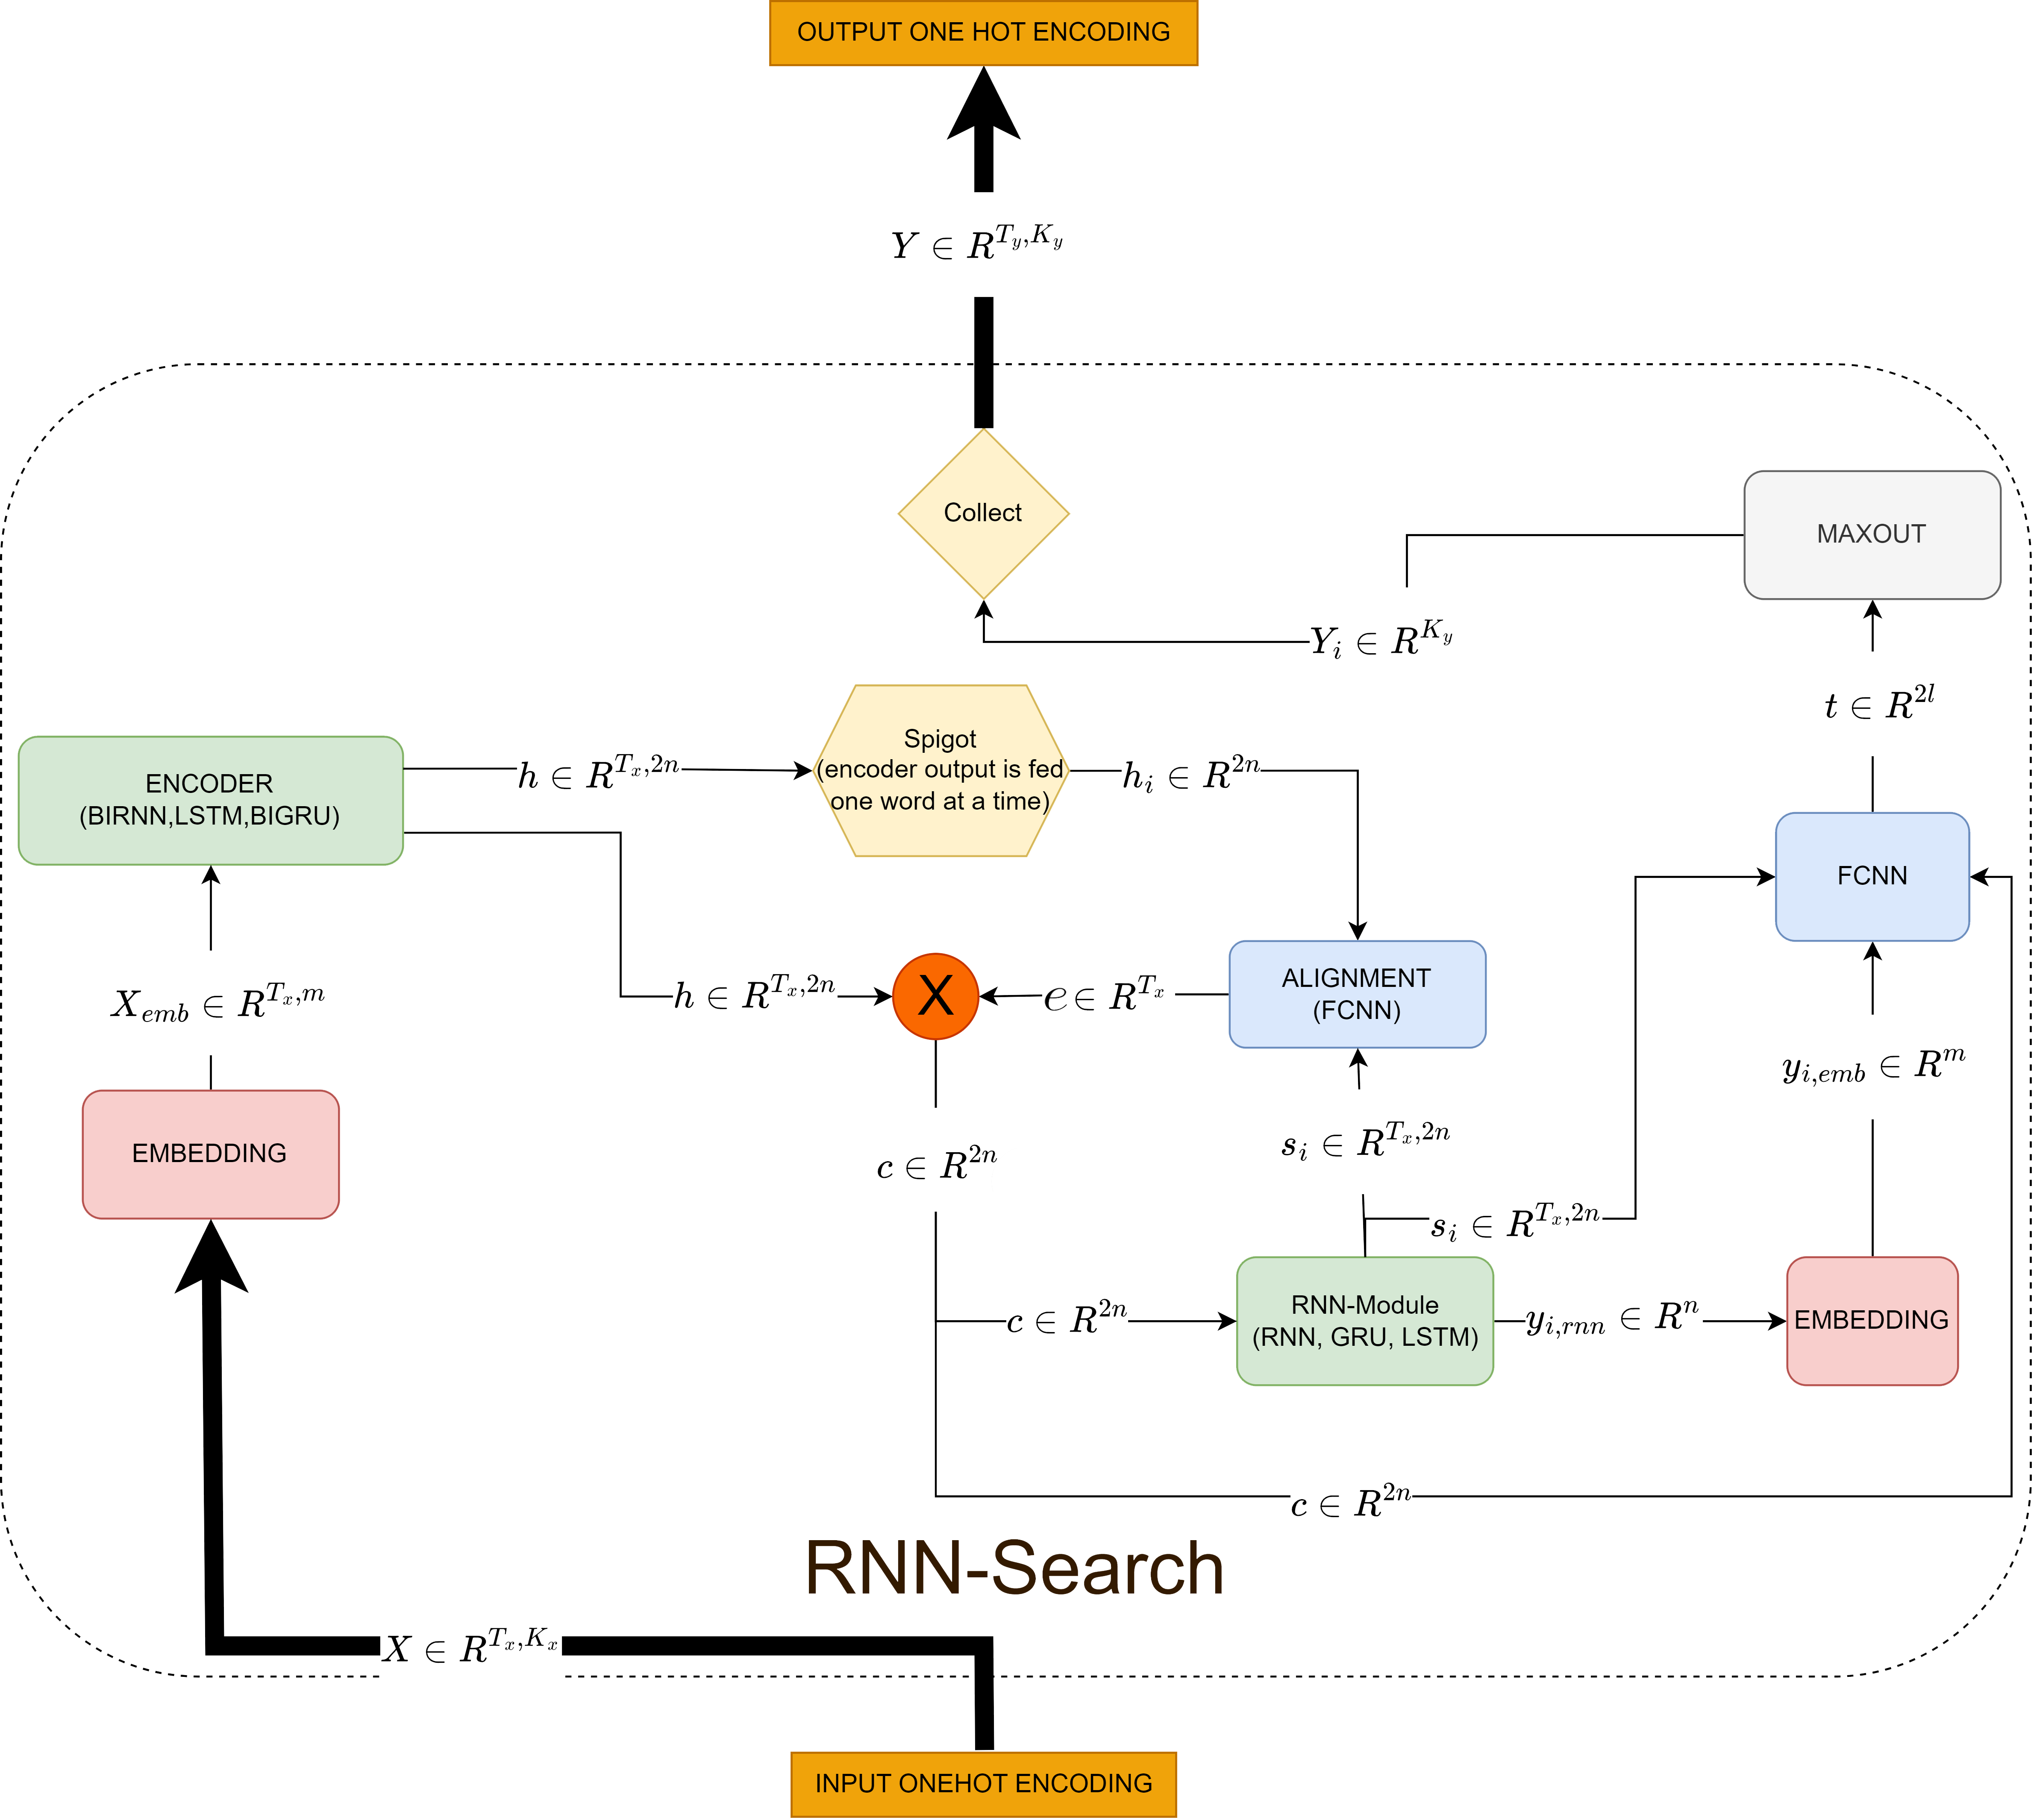
\includegraphics[width=\textwidth]{architecture.png}
    \caption{General Presentation of the Used architecture}
    \label{fig:architecture}
\end{figure}

In my approach, I tried to be as close as possible to the article's proposed architecture \ref{fig:architecture}. The model was organized into two main modules: An encoder and a decoder. On one hand, the encoder takes one-hot encoding representation of the input English phrase, reduces its dimension, then applies an RNN type module. On the other hand, the decoder takes the sequence of vectors given by the encoder, and one vector at a time calculates some weights to be used to modify the input vectors into one context vector that is used to predict the current word after being passed through a maxout layer.



\subsection{Approach Overview}

The paper introduces an innovative approach to enhance existing machine translation models, diverging from both statistical models and Encoder-Decoder architectures. The approach can be divided into the following substeps:

\subsubsection{Phrase Encoding}

The initial step involves encoding the input phrase using a Bag-of-Words representation. The vocabulary for this representation is derived either from the web, encompassing the most common 30,000 English/French words, or by utilizing the training set alone, or in combination with the test set. Each word in a phrase is then represented by indices in the vocabulary. Words without corresponding entries in the current vocabulary are mapped to the \textbf{\textless UNK\textgreater} token. Sentence padding is applied without an \textbf{\textless EOS\textgreater} token index, with the expectation that the model learns when to conclude. Consequently, each phrase is represented by a tensor of size $R^{T_x}$.

\subsubsection{Embedding and Encoding}

For efficient preprocessing, multiprocessing (except on Linux due to incompatibility) and HuggingFace's \textbf{.map} method are employed, significantly expediting data processing. The representation undergoes transformation through an embedding layer, resulting in a vector of size $R^{T_x,m}$. This vector is directly fed into the Bi-RNN unit of the encoder, producing an output of size $R^{T_x,2n}$ and an unused hidden state.

\subsubsection{Decoding and Maxout}

In a sequential manner, the encoder's output vectors $h_i$ are fed into the decoder module. Initially, the Alignment network generates weights of size $R^{T_x}$. These weights combine the $h$ vectors into a context vector $c$, which is then supplied to the RNN section of the decoder. Post-decoding, the hidden state of the RNN, its output $y_{i,rnn}$ (compressed to the size of the embedding $m$), and the context vector are processed through a single Fully Connected layer. Subsequently, the output undergoes a max-out layer, halving its dimension, followed by a "relaxation" layer to achieve the desired shape of $R^{K_y}$. This representation signifies the probability of $y_i$ representing each word in the vocabulary, with the omission of softmax until the application of the Negative Log Loss in the loss criterion. After predicting $y_i$ for $i \in [1:T_y]$, we backpropagate the loss along with L2 regularization loss taken with respect to all model parameters.

\subsection{Detailed Architecture}

We'll be using the following notations: $T_x, T_y$ sequence length of input and output respectively. $K_x, K_y$ vocabulary sizes used for input and output respectively. $m$ is the embedding size, $n$ is the hidden dimension size in both the encoder's RNN and that of the decoder, and $l$ is a latent dimension used in the MaxOut module.
\subsubsection{RNNSearch Translation Model}
\begin{enumerate}
    \item \textbf{Embedding layers ($E_1$ and $E_2$)}: used to reduce the dimension of the input one-hot encoded vector from $T_x$, can be represented by two 2D matrices or a single dense layer with no activation function and no bias.
    
    \item \textbf{Encoder's BiRNN layer (We use GRU as the RNN module)}: We do not directly use the hidden state of the encoder, only the output of size $R^{T_x,2n}$.
    
    \item \textbf{Alignment network}: The main contribution of the paper. Used to calculate the weights corresponding to each part of the sentence $\in R^{T_x}$. Uses the current hidden state of the decoder's RNN and the corresponding decoder's output.
    
    \item \textbf{Decoder's RNN}: used in a one-step-at-a-time fashion (feeding only sequences of length 1) to be able to modify the next input with a context vector generated from the alignment network.
    
    \item \textbf{Maxout Unit}: combines outputs from the decoder's RNN, the predicted word, and the context vector. It implements the maxout activation with two units as described in \cite{Goodfellow-et-al-2016}.
\end{enumerate}
\subsubsection{RNNEncoDeco Translation Model}
We by pass all connections used previously in RNNSearch and directly apply the RNN layer of the decoder to the encoder's output then apply a "relaxation" layer and a softmax to get the probabilities of predicting a word in the vocabulary.

\subsection{Training}

\begin{enumerate}
    \item \textbf{Cost Function:} We experiment with both : Negative log-likelihood and Cross Entropy Loss. To that we add an L2 regularization over all the parameters of the model with a weight of $10^{-4}$
    
    \item \textbf{Optimization}: Since Adadetla used in the article is a special case of Adam without the first order smoothing, we expirement with both.
    
    \item \textbf{Checkpointing:} we save a copy of our model everytime the loss on the validation gets smaler after an entire epoch

    \item \textbf{Framework:} We completely rely on pytorch for it's compatibality and ease of use. 
    
    \item  \textbf{Unitary Testing:} For each of the implemented modules we implement a corresponding unit test that insures types, intialization and tensor shapes. 
    
\end{enumerate}

\subsection{Inference (Translation)}

when it comes to predicting phrases, we rely on an optimized version of beam search that implements rejection of consecutive parts repition within a sentence with beam length of 5.
We also tried with argmax to predict indicies but results weren't always coherent



% DATA section
\section{Dataset}
\label{sec:data}
HuggingFace provides the  WMT ’14 dataset containing about 40M sentences totaling around 800M individual words. 
We do not apply the dataselection method described by the article and we limit ourselves to the first 4M phrases for the training set and the test set of 3k samples provided by huggingface. 

The dataset contains mostly political news.
Ex: 
\begin{enumerate}
    \item English:  The city is mentioned in ancient Greek and ancient Egyptian legends.
French:  La ville est mentionnée dans les légendes grecques et égyptiennes de l'Antiquité.
\item English:  We want to look 5-10 years into the future and predict cardinal changes in this interaction.
French:  Nous voulons regarder 5 à 10 ans devant nous et deviner les changements radicaux qui se produiront avec cette interaction.
\end{enumerate}



% EXPERIMENT section
\section{Evaluation}
\label{sec:experimence}
\subsection{Hyperparameter Tuning}

The optimization of our model's performance involved meticulous adjustments to specific hyperparameters. The following configurations were explored and refined during the fine-tuning process:

\begin{enumerate}
    \item \textbf{Batch Size:} Experimentation with batch sizes ranging from 80 to 256 was conducted during training. Smaller batches proved to induce chaotic behavior in some cases when using SGD.
    
    \item \textbf{Optimizer:} For Adam, the initial learning rate was set to $0.001$, while Adadelta utilized a learning rate of $1.0$, $\epsilon=10^{-6}$, and $\rho=0.95$.
    
    \item \textbf{Dataset Size:} After shuffling, we limit the enormous dataset to around 4 million translation examples, equivalent to approximately 60 million words. Additionally, we limit our expirements to $T_x=T_y=15$ as the original paper shows significant divergence at this point when it comes to bleu score. 
    
    \item \textbf{Dropout Layers:} Dropout layers with a 20\% probability were incorporated into the decoder RNN module and the Fully Connected layer used for maxout.
    
    \item \textbf{Batch Normalization:} A single layer with the number of features equal to $T_x$ was added at the output of the encoder.
    
    \item \textbf{Gradient Clipping:} All gradients were clipped to have a norm at most 1.0, following the approach outlined in the paper.
    
    \item \textbf{L2 Regularization:} To address loss explosions, especially on the university's GPU, L2 regularization was introduced, mitigating numerical precision errors not observed on local GPUs.
\end{enumerate}

\subsection{Training Process Overview}

The training process involved several crucial components:

\subsection{Experimental Setup}

The following experimental setup was used for training and evaluation:

\begin{enumerate}
    \item \textbf{Evaluation Frequency:} The model was evaluated on a complete dataset of 3000 samples. Four randomly chosen examples were translated using the beam search algorithm. A threshold on log probabilities (-2.8) was used to control the generation process, stopping the generation of next words if the maximum log probability dropped below the threshold.
    
    \item \textbf{Hardware:} Training was performed on both local hardware with Windows 11 and an Nvidia RTX 3080 (8GB VRAM) portable GPU, as well as the university's Linux servers equipped with Nvidia Quadro RTX 6000 (24GB VRAM).
    
    \item \textbf{Epochs:} For smaller databases (around 100K examples), approximately 20 epochs were executed. The larger dataset of 4 million examples required an extended training period of 6 epochs to capture complexity and patterns comprehensively.
    
    \item \textbf{Training Time:} Each model was trained for approximately 20 hours to achieve the final results.
\end{enumerate}

\subsection{Metrics}

The cost function employed was Negative-Log-Loss, producing initial losses around 10 and concluding at approximately 2 during training. Additionally, the Bleu score, which assesses repetitions of sequences of a fixed length $k$ (with $k=3$ in our experiments), was used to compare phrases.


\subsection{Results}

This section presents the outcomes of our endeavor to reimplement a noteworthy paper. Due to some vague details, adaptations were made by adding or removing functionalities. Two models, RNNsearch-20 and RNNEncDeco-20, were trained for around 6 epochs. The first figure compares the translation performance of the two models for a phrase of size 20, evaluating the mean Bleu score for both translations and the expected one.

\subsection{Discussion}

During the implementation of our enhanced encoder-decoder model with attention mechanism, we encountered several challenges and limitations that affected our results.

One major challenge was the issue of overfitting due to the use of a smaller vocabulary size and a limited dataset. This resulted in significant deviations from the results reported in the original paper. We attempted to address this problem by adjusting various components of the model, such as reducing the embedding size and modifying the hidden size of the output network. However, finding the optimal combination of hyperparameters proved to be a time-consuming process.

Another limitation of our implementation was the lack of data selection, as described in the original paper. Due to time constraints, we were unable to implement this crucial step, which could have significantly improved our results by extracting more relevant data from the dataset.

Furthermore, the limited training time of only 6 epochs and the constraint of a smaller dataset also impacted our results. We were unable to train the model for longer periods or with larger datasets, which may have affected the model's ability to capture complex patterns comprehensively.

Additionally, since we implemented everything from scratch, we encountered several bugs and inconsistencies between our implementation and the details provided in the original paper. These challenges further hindered our progress and affected the accuracy of our results.

Overall, while we made efforts to enhance the basic model and address the challenges we encountered, the limitations and constraints we faced had a significant impact on the performance of our model.


% CONCLUSION section
\section{Conclusion}
\label{sec:conclusion}
In this project, we successfully achieved promising results within the given time limit. Our implemented model effectively translates English sentences to French with a satisfactory level of accuracy, despite occasional repetition in the generated output. The alignment figures obtained closely resemble those presented in the referenced paper, indicating that our model is on the right track to function as intended.

To enhance the convergence speed of the model, we experimented with various techniques. Additionally, we explored different approaches to improve the quality of the generated sentences. We believe that by training the same architecture for a longer duration and with more data, we can achieve results comparable to those reported in the referenced paper.

\subsection{Challenges and Limitations}
Reimplementing a complex architecture from scratch presented its challenges. We had to make numerous assumptions and decisions, leading to a significant amount of trial and error. However, this project provided us with valuable insights into attention models, which we have been interested in since studying them in class. Overall, we are pleased to have participated in this project and gained a deeper understanding of how attention models function.


% % BIBLIO section
% \section{Bibliographie}

% \textbf{Bibliographie : une liste complète des principaux articles de l'état de l'art ou ayant inspiré la démarche, et qui seront référencés de manière pertinente dans le rapport.}\\

% Par exemple \citep{Goodfellow-et-al-2016} et \citep{test}


\bibliography{biblio}

\end{document}

